\documentclass{article}
\usepackage[utf8]{inputenc}
\usepackage[spanish]{babel}
\usepackage{listings}
\usepackage{graphicx}
\graphicspath{ {images/} }
\usepackage{cite}

\begin{document}

\begin{titlepage}
    \begin{center}
        \vspace*{1cm}
            
        \Huge
        \textbf{Proyecto final}
            
        \vspace{0.5cm}
        \LARGE
        Informática II
            
            
        \vspace{1.5cm}
        
        \textbf{Marcela Flórez Orellano} 
        
        \vspace{0.3cm}
        \LARGE
        
        \textbf{Ferney Mejía Pérez}
            
        \vfill
            
        \vspace{0.8cm}
            
        \Large
        Departamento de Ingeniería Electrónica y Telecomunicaciones\\
        Universidad de Antioquia\\
        Medellín-Antioquia\\
        Octubre de 2021
         
            
    \end{center}
\end{titlepage}


\tableofcontents
\newpage


\section{Sección introductoria}\label{intro}
El presente proyecto hace énfasis en la implementación de las ideas principales del proyecto final correspondiente al curso en proceso, informática II, la cual tiene un enfoque de enseñanza en el lenguaje de programación C++, de tal motivo que, se realizarán diversos ejercicios de aprendizaje con el fin de adquirir lógica computacional y la habilidad necesaria para la solución de problemas comunes en la programación. Por lo tanto, para este proyecto se tiene de inicio la creación del esquema organizacional del cual se desprenderán las diferentes ideas que componen el cuerpo del juego correspondiente al mencionado proyecto.

La finalidad del juego a desarrollar es que el usuario pueda competir en diferentes galaxias para ser el mejor piloto intergaláctico del universo conocible, esto se logra derrotando al ejército de enemigos galácticos y su jefe "Galactic Burglar". Se cuenta con dos niveles de diferentes mapas cada uno, en los que los contenidos galácticos cambian igual que los enemigos. Además, el juego presenta la opción de multijugador, específicamente para dos jugadores.

\section{Sección de contenido} \label{contenido}
A continuación se presentan las ideas pertenecientes al esquema organizacional del juego:

\subsection{Entorno}
El juego tendrá un entorno desarrollado en el espacio sideral, en el cual habrá múltiples galaxias a las cuales acceder para realizar competiciones en un mínimo de tiempo de tres minutos por nivel. 

En la introducción del juego se podrá presenciar el nombre del videojuego y el botón de inicio:


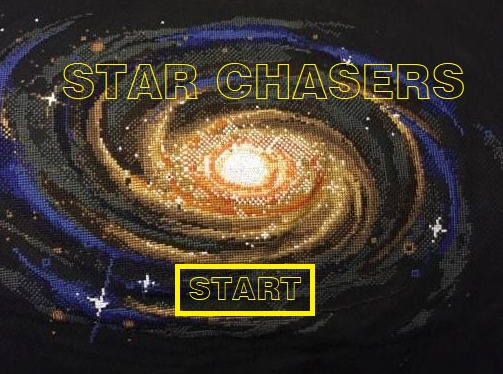
\includegraphics[scale=0.59]{Ideación/Images/Start.jpeg}


En general se podrá presenciar en la parte superior del mapa el tiempo, el nivel y el número de vidas que posee el jugador. 

EL fondo para el nivel 1: 

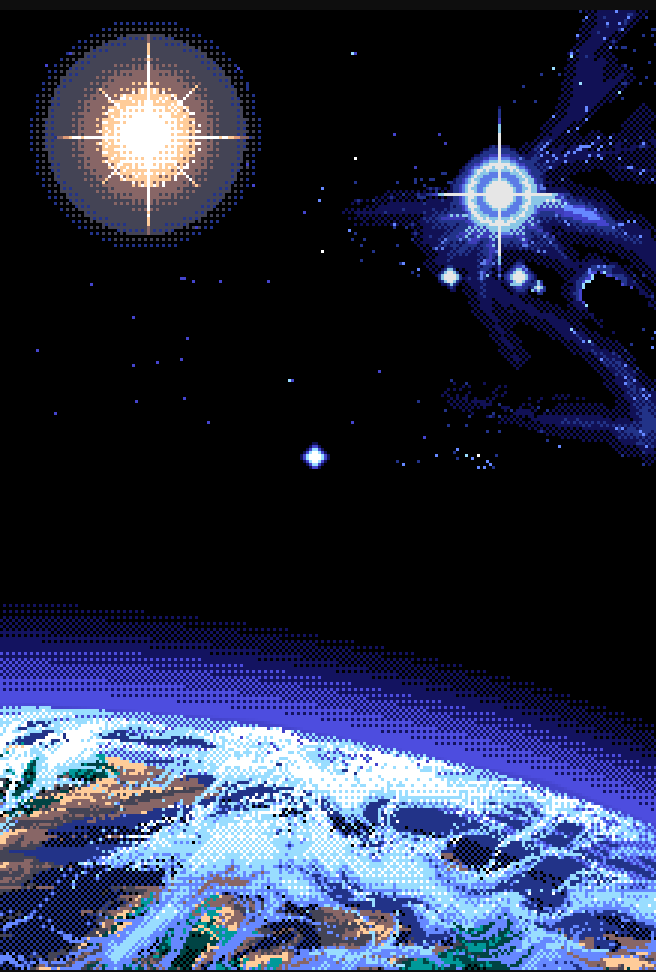
\includegraphics[scale=0.40]{Ideación/Images/mapa1.png}

El fondo para el nivel 2:

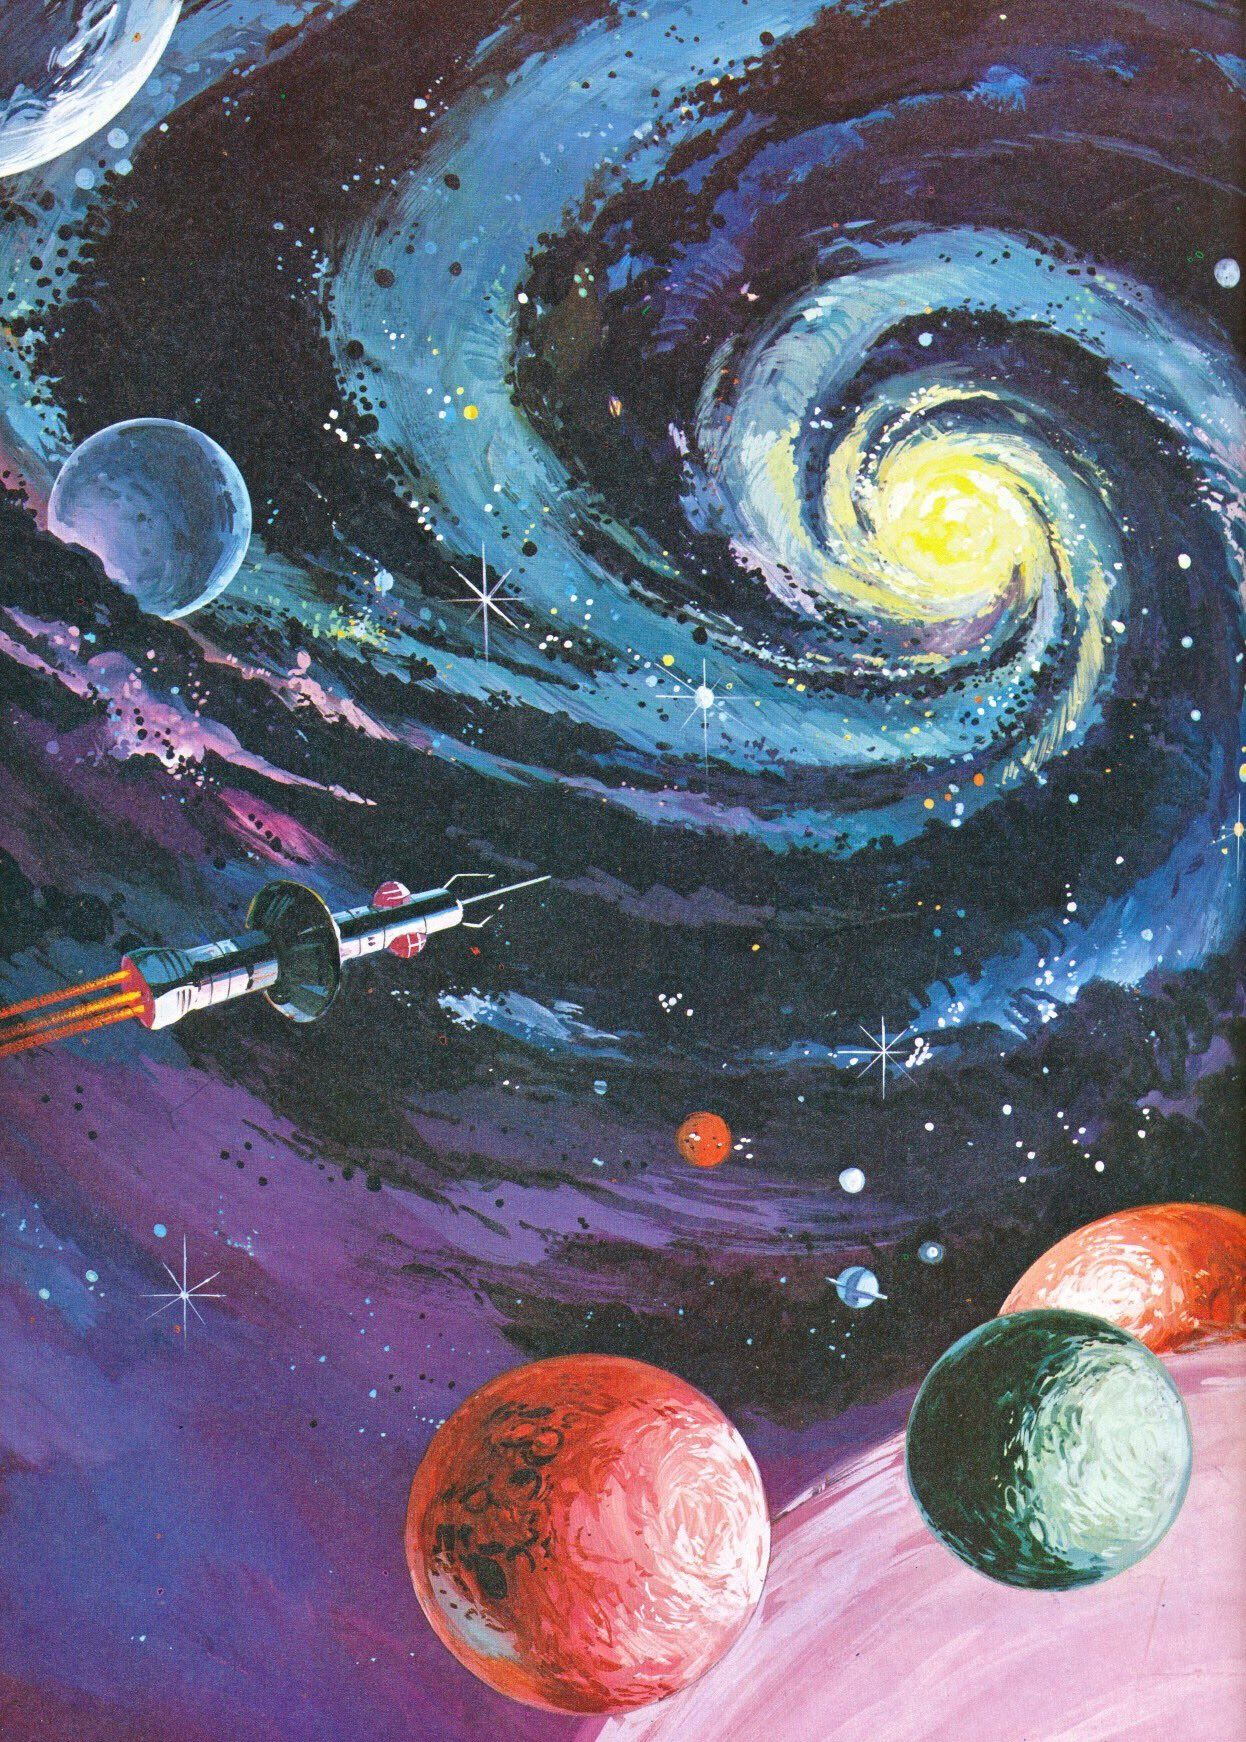
\includegraphics[scale=0.21]{Ideación/Images/mapa2.jpeg}

Además, la visualización del personaje moviéndose en el mapa será de manera vertical y horizontal, describiendo el tipo de movimiento presentado en la siguiente imagen:  

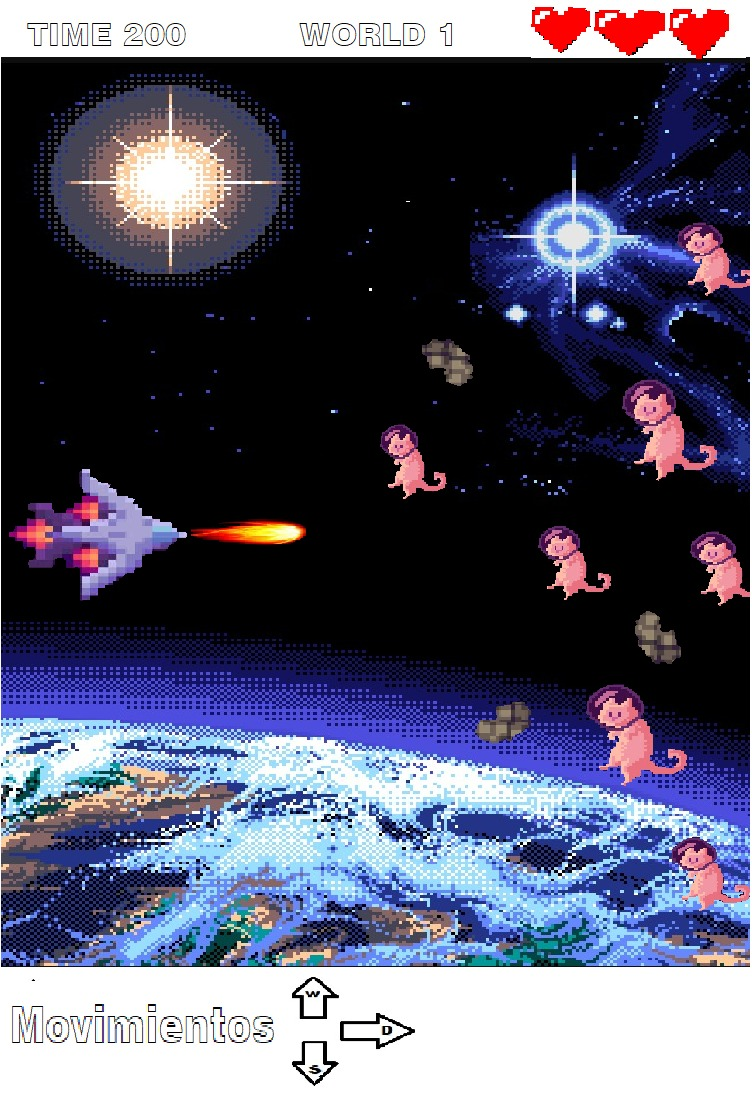
\includegraphics[scale=0.35]{Ideación/Images/movimientos.jpeg}


\subsection{Protagonistas}
Se contarán con algunos personajes que se encuentran en búsqueda de ser los mejores exploradores intergalácticos, los cuales dispondrán de varias naves con tecnología cuántica capaz de sobrepasar las leyes de la física, que a su vez la diversidad de los niveles y mapas permitirán conocer nuevos confines galácticos con mayores dificultades. 

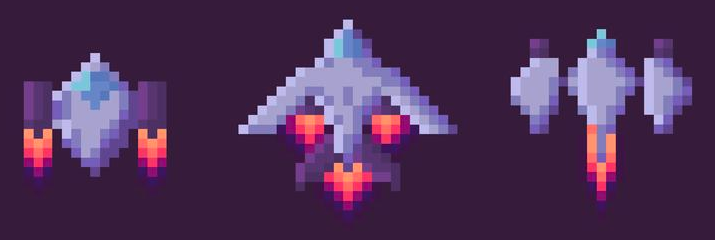
\includegraphics[scale=0.48]{Ideación/Images/protagonistas.png}

\subsubsection{Antagonistas}
Criaturas desconocidas que aumentan su poder y capacidad de ataque a medida que se avanza de nivel. Estos monstruos aparecerán de forma aleatoria a lo largo del juego, con el objetivo de interferir con la exploración de los personajes principales. Cabe anotar que, durante los diferentes niveles aparecerán diferentes personajes de la armada galáctica de saqueadores comandados por un jefe final conocido en el oscuro universo como "Galactic Burglar". 

Los personajes de la armada no efectuarán disparos hacia los personajes principales, sin embargo, si llega haber un contacto entre los protagonistas y los antagonistas se les reducirá las vidas a los personajes principales. 

Por último, el jefe final podrá disparar bombas de energía a la velocidad de la luz que, si colisionan 5 veces con los personajes principales, los destruirán inmediatamente. 

Enemigo 1: 



\includegraphics[scale=0.55]{Ideación/Images/enemigo.png}

Enemigo 2:

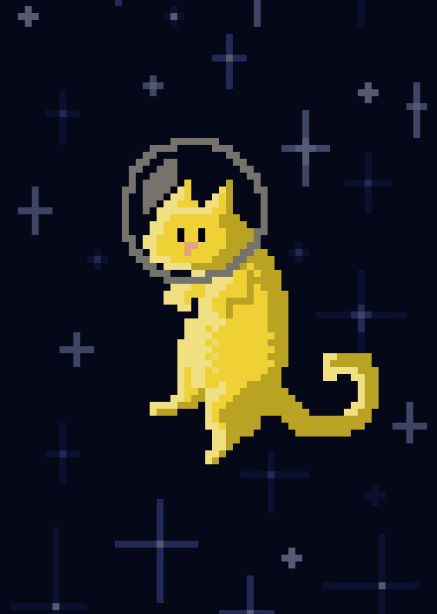
\includegraphics[scale=0.30]{Ideación/Images/enemigo2.png}

Jefe final: 



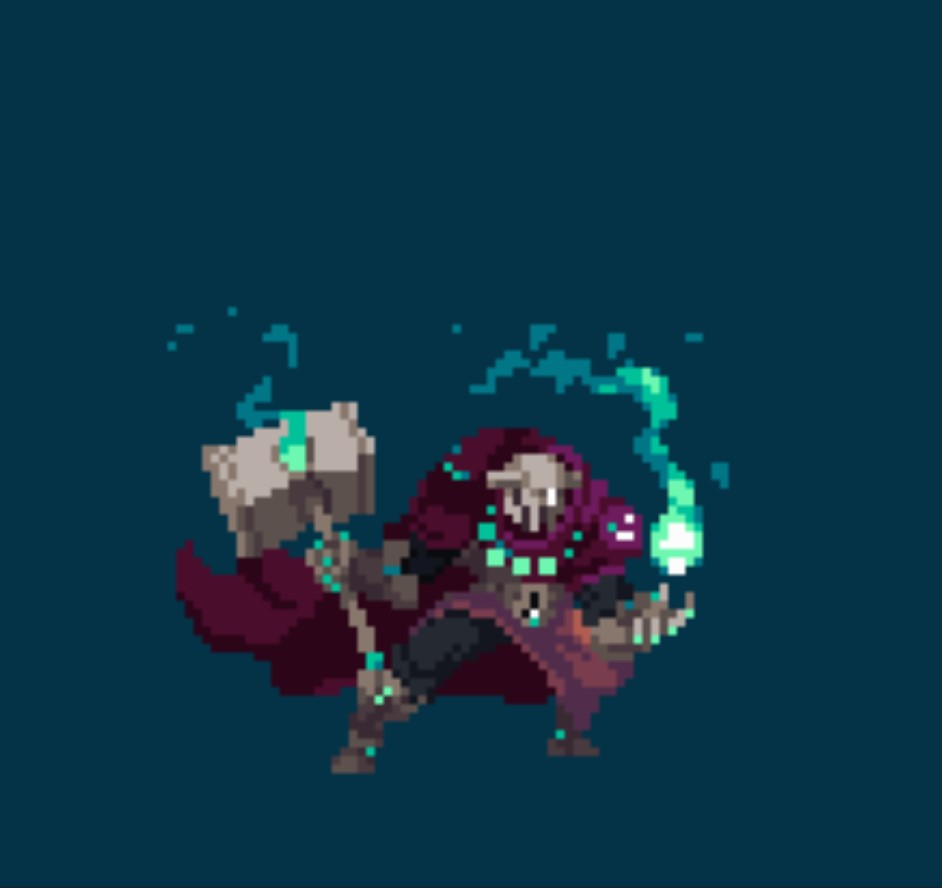
\includegraphics[scale=0.28]{Ideación/Images/jefe_final.jpg}


\subsection{Acciones}
Los jugadores se enfrentarán a la armada galáctica de saqueadores a los cuales se les podrá disparar rayos cósmicos y poder terminar con la vida de los mismos, permitiendo el avance a través del mapa.

\subsection{Recursos}
A lo largo del juego se encontrarán meteoritos que estarán orbitando de manera circular, los cuales tendrán posibles poderes escondidos dentro de ellos que le otorgaran a los jugadores la capacidad de eliminar a todo el ejército de enemigos y pasar directamente a la fase de combate con el jefe final, el segundo es el de poder de atravesar por un agujero de gusano, tratándose de un atajo para alcanzar la meta y así subir de nivel. 
Para obtener el poder, el usuario deberá disparar y hacer explotar el meteorito.

\subsection{Eliminación}
Los jugadores cuentan con tres vidas, si estos son atacados por los enemigos, o si no cumplen con el tiempo estipulado se reinicia automáticamente el nivel el juego y se les quita una vida. El juego finaliza si los jugadores pierden todas sus vidas.

\subsection{Interacción}
Para la opción de un único jugador, el movimiento del personaje estará controlado por las teclas W para arriba y S para abajo. Si se escoge de tipo multijugador estas mismas teclas se usaran para el jugador 1 y las teclas de las flechas arriba y abajo se usaran para el jugador 2.


El jugador podrá eliminar a las criaturas que irán emergiendo mientras se recorren las pistas galácticas con la tecla R. Para tipo multijugador se usaran la tecla R para el jugador 1 y la tecla P se usara para el jugador 2.

\subsection{Modalidad}
El juego estará diseñado para la jugador individual o multijugador, quienes podrá elegir distintas naves intergalácticas.

\subsection{Dificultad}
Mientras más avanza el jugador en las diferentes galaxias, más irá costando el ganar dentro de los diferentes mundos de acción, es decir, el nivel de dificultad aumentará pese tenga más recorrido y haya sobrepasado niveles inferiores. 

\subsection{Esquema de las clases a implementar}

\subsubsection{Registro y lectura de datos}
Esta clase tiene como objetivo almacenar la información de los usuarios, es decir, su "nickname" y contraseña, se tiene pensado usar -----

Para darle inicio al juego se visualizará una ventana con las opciones para ingresar o crear un nickname.

\subsubsection{Clase matriz }
Esta clase tiene como objetivo generar el espacio del juego.

\subsubsection{Clase personaje}

En esta clase se podrá generar el movimiento de los personajes dentro del mapa a partir de las teclas presionadas por el usuario. Se tendrá una función para la rutina de muerte la cual se activa al momento de ser tocados por los enemigos, también se encontrara la definición de los poderes que se podrán utilizar a lo largo del juego. 
\subsubsection{Clase matriz}
Esta clase tiene como objetivo generar el espacio del juego.
\subsubsection{Clase meteorito}
\subsubsection{Clase proyectil}

\newpage

\bibliographystyle{IEEEtran}
\bibliography{references}
\cite{calistenia}


\end{document}
